%-----CLASS LOADING-------------------
\ifx\pdfoutput\undefined
\documentclass[a4paper,twoside,12pt,dvips]{article}
\else
\documentclass[a4paper,twoside,12pt,pdftex]{article}
\fi

%-----LANGUAGE SELECTION-------------
\usepackage[english]{babel}
\selectlanguage{english}

\usepackage{graphicx,color,hyperref,fancyhdr,longtable,listings,multirow}

%-----CONFIG HYPERREF-----------------
\definecolor{rltred}{rgb}{0.75,0,0}
\definecolor{rltgreen}{rgb}{0,0.25,0}
\definecolor{rltblue}{rgb}{0,0,0.75}
\hypersetup{colorlinks=true,
  urlcolor=rltblue,                % \href{...}{...} external (URL)
  filecolor=rltgreen,              % \href{...} local file
  linkcolor=rltred,                % \ref{...} and \pageref{...}
  bookmarks         = true,        % Signets
  bookmarksnumbered = true,        % Signets numerotes
  pdfpagemode       = UseOutlines, % Signets/vignettes ferme a l'ouverture
  pdfstartview      = FitV,        % La page prend toute la largeur
  pdfpagelayout     = OneColumn,   % Vue par page
  pdfborder         = {0 0 0},     % Style de bordure : ici, pas de bordure
  pdftitle          = {Syndicate file format},
  pdfauthor         = {Paul CHAVENT},
  pdfsubject        = {Syndicate file format},
  pdfkeywords       = {bullfrog syndicate 1993 file format}
}

%-----CONFIG LISTINGS-----------------
\lstset{language=C, frame=single, showstringspaces=false, xleftmargin=12pt, numbersep=8pt, numberstyle=\tiny, stepnumber=1}
%framerule=0pt,backgroundcolor=\color{grisclair},frame=none,numbers=left

%-----MISE EN PAGE--------------------
%-header and footer-
\pagestyle{fancy}
\rhead[~]{~}
\chead[~]{~}
\lhead[{\small libsyndicate}]{~}
\lfoot[\textbf{\thepage}]{~}
\cfoot[~]{~}
\rfoot[\today]{ \textbf{\thepage} }
\renewcommand{\headrulewidth}{0.2pt}
\renewcommand{\footrulewidth}{0.2pt}

%-paragraphs
\setlength{\parindent}{0in}
%\renewcommand{\baselinestretch}{1.1}
\setlength{\parskip}{0.2\baselineskip}

%-margins- A4 = 297 x 210 mm = 11.7 x 8.3 inches (1in~2.2cm)
% http://www.ctan.org/tex-archive/macros/latex/contrib/fancyhdr/fancyhdr.pdf
% http://www.iam.ubc.ca/~newbury/tex/page-set-up.html
\setlength{\hoffset}{0in}
\setlength{\oddsidemargin}{0in}
\setlength{\evensidemargin}{0in}
\setlength{\textwidth}{6.3in} % 6.3in (16cm) (1in on each side)
\setlength{\linewidth}{\textwidth}
\setlength{\headwidth}{\textwidth}

\setlength{\voffset}{-0.75in}
\setlength{\topmargin}{0in}
\setlength{\headheight}{0.5in}
\setlength{\headsep}{0.25in}
\setlength{\textheight}{9.7in} % 9.7in (22cm) (1in on the top and bottom)
\setlength{\footskip}{0.75in}

% 8<-----DOCUMENT------------------------
\begin{document}

% 8<-----FIRST PAGE----------------------
\begin{titlepage}
  ~\vfill
  \begin{center}
    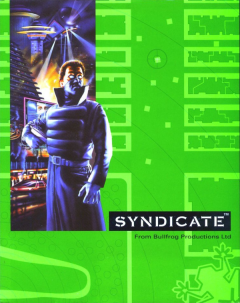
\includegraphics{picts/SyndicateCover}\vspace{1.5cm}\\
    {\LARGE Syndicate file format}\\
    {\small (This is the reference for coding libsyndicate)}\\
  \end{center}
  \vspace{1.5cm}  
  \begin{flushright}
    \today
  \end{flushright}
  \vfill
\end{titlepage}

% 8<-----SECOND PAGE---------------------
\thispagestyle{empty}
\begin{center}
The libsyndicate project is in no way affiliated with Electronic Arts and/or Bullfrog Entertainment.\\
Syndicate and Bullfrog are trademarks of Electronic Arts.\\
Syndicate is \copyright{} 1993 Electronic Arts.
\end{center}
\vfill

\newpage

% 8<-----SUMMARY-------------------------
\tableofcontents
\newpage
\makeatletter
\if@twoside
 \ifodd\c@page~\newpage
 \fi
\fi
\makeatother

% 8<-----INTRODUCTION--------------------
\section{Introduction}

This is a documentation that resume informations that was needed to code the libsyndicate.

Thanks to :
\begin{itemize}
\item \href{http://www.yoda.arachsys.com/dk/utils.html}{Jon skeet for dernc}.
\item \href{http://citybuilder.sourceforge.net/}{Andrew Sampson for the first reverse ingenering of graphic files}.
\item \href{http://desyndicate.pbwiki.com/}{Marcin Olak and the Desyndicate wiki}.
\item \href{http://freesynd.sourceforge.net/about.php}{Stuart Binge, Joost Peters, Trent Waddington and the freesynd project staff}.
\item \href{http://syndicate.lubie.org/siteinfo/contact.php}{Tomasz Lis for his fan site that resume the whole above}.
\item \href{ftp://ftp.mplayerhq.hu/MPlayer/samples/game-formats/magiccarpet-fli/}{Mike Melanson for details on fli files}.
\end{itemize}

The author of this document is Paul Chavent (valefor at icculus dot org).


The Syndicate version covered by this document is the one for PC.


% 8<-----LIST OF FILES AND TYPES---------
\section{List of files and types}
\label{sec:files_and_types}

\subsection{List of data files}
\label{sec:files}

This is a list of files with the type of data. Types of data are defined in section~\ref{sec:types}.

The prefix 'h' could mean Hight resolution. For example there are \texttt{HPOITNER.DAT} and \texttt{LPOINTER.DAT}.

The prefix 'm' could mean menu.

The prefix 'i' could mean intro.

\begin{center}
  \begin{longtable}{|l|l|l|}

    \hline \textbf{File} & \textbf{Type} & \textbf{Comment} \\ \hline 
    \endfirsthead

    \hline \textbf{File} & \textbf{Type} & \textbf{Comment} \\ \hline 
    \endhead

    COL01.DAT    & MapColumn     & Gives the type for each of the 256 tiles \\
    \hline
    GAME[xx].DAT & Game          & The description of the games \\
    \hline
    HBLK01.DAT   & MapTile       & The 256 base tiles that compund maps \\
    \hline
    HELE-0.ANI   & SpriteElement & The descriptions of sprite elements \\
    \hline
    HFNT01.DAT   & Font          & FIXME : don't know for what is it used ?\\
    \hline
    HFRA-0.ANI   & SpriteFrame   & The descriptions of sprite frames \\
    \hline
    HPAL01.DAT   & Palette       & \multirow{5}{*}{palettes for maps} \\ 
    \cline{1-2}
    HPAL02.DAT   & Palette       & ~ \\ 
    \cline{1-2}
    HPAL03.DAT   & Palette       & ~ \\ 
    \cline{1-2}
    HPAL04.DAT   & Palette       & ~ \\ 
    \cline{1-2}
    HPAL05.DAT   & Palette       & ~ \\ 
    \hline
    HPALETTE.DAT & Palette       & FIXME \\
    \hline
    HPOINTER.DAT & SpriteData    & \multirow{2}{*}{arrow, pick, target, pointers} \\
    \cline{1-2}
    HPOINTER.TAB & SpriteTab     & ~ \\ 
    \hline
    HREQ.DAT     & GameFont      & Fonts used for the game screen \\
    \hline
    HSPR-0.DAT   & SpriteData    & \multirow{2}{*}{sprites for maps} \\
    \cline{1-2}
    HSPR-0.TAB   & SpriteTab     & ~ \\ 
    \hline
    HSTA-0.ANI   & SpriteAnim    & The descriptions of sprite anims \\
    \hline
    INTRO.DAT    & Fli           & Animation for the introduction \\
    \hline
    INTRO.XMI    & Music         & Music for the introduction \\
    \hline
    ISNDS-0.DAT  & SoundData     & FIXME \\
    \hline
    ISNDS-0.TAB  & SoundTab      & FIXME \\
    \hline
    ISNDS-1.DAT  & SoundData     & FIXME \\
    \hline
    ISNDS-1.TAB  & SoundTab      & FIXME \\
    \hline
    MAP[xx].DAT  & MapData       & Map data (tiles reconstitution) \\
    \hline
    MBRIEF.DAT   & Fli           & ~ \\
    \hline
    MBRIEOUT.DAT & Fli           & ~ \\
    \hline
    MCONFOUT.DAT & Fli           & ~ \\
    \hline
    MCONFUP.DAT  & Fli           & ~ \\
    \hline
    MCONSCR.DAT  & Raw           & ~ \\
    \hline
    MDEBRIEF.DAT & Fli           & ~ \\
    \hline
    MDEOUT.DAT   & Fli           & ~ \\
    \hline
    MENDLOSE.DAT & Fli           & ~ \\
    \hline
    MENDWIN.DAT  & Fli           & ~ \\
    \hline
    MFNT-0.DAT   & SpriteData    & \multirow{2}{*}{The menu fonts (rle encoded)} \\
    \cline{1-2}
    MFNT-0.TAB   & SpriteTab     & ~ \\
    \hline
    MGAMEWIN.DAT & Fli           & ~ \\
    \hline
    MISS[xx].DAT & Mission       & Defines the mission objectives etc.\\
    \hline
    MLOGOS.DAT   & Raw           & ~ \\
    \hline
    MLOSA.DAT    & Fli           & ~ \\
    \hline
    MLOSAOUT.DAT & Fli           & ~ \\
    \hline
    MLOSEGAM.DAT & Fli           & ~ \\
    \hline
    MMAP.DAT     & Fli           & ~ \\
    \hline
    MMAPBLK.DAT  & Raw           & ~ \\
    \hline
    MMAPOUT.DAT  & Fli           & ~ \\
    \hline
    MMINLOGO.DAT & Raw           & ~ \\
    \hline
    MMULTI.DAT   & Fli           & ~ \\
    \hline
    MMULTOUT.DAT & Fli           & ~ \\
    \hline
    MOPTION.DAT  & Fli           & ~ \\
    \hline
    MOPTOUT.DAT  & Fli           & ~ \\
    \hline
    MRESOUT.DAT  & Fli           & ~ \\
    \hline
    MRESRCH.DAT  & Fli           & ~ \\
    \hline
    MSCRENUP.DAT & Fli           & ~ \\
    \hline
    MSELECT.DAT  & Fli           & ~ \\
    \hline
    MSELECT.PAL  & Palette       & Palette for the menus \\
    \hline
    MSELOUT.DAT  & Fli           & ~ \\
    \hline
    MSPR-0.DAT   & SpriteData    & \multirow{2}{*}{The menu sprites (rle encoded)} \\
    \cline{1-2}
    MSPR-0.TAB   & SpriteTab     & ~ \\
    \hline
    MTITLE.DAT   & Fli           & ~ \\
    \hline
    SAMPLE.AD    & Audio/sound   & ~ \\
    \hline
    SAMPLE.OPL   & Audio/sound   & ~ \\
    \hline
    SOUND-0.DAT  & SoundData     & ~ \\
    \hline
    SOUND-0.TAB  & SoundTab      & ~ \\
    \hline
    SOUND-1.DAT  & SoundData     & ~ \\
    \hline
    SOUND-1.TAB  & SoundTab      & ~ \\
    \hline
    SYNGAME.XMI  & Music         & ~ \\
    \hline

    \caption[Table of files]{Table of files.} \label{tab:files} \\

  \end{longtable}
\end{center}

\subsection{List of data types}
\label{sec:types}

This is a list of types.

\begin{center}
  \begin{longtable}{|l|c|p{0.6\linewidth}|}

    \hline \textbf{Type} & \textbf{Reverse} & \textbf{Files associated} \\ \hline 
    \endfirsthead

    \hline \textbf{Type} & \textbf{Reverse} & \textbf{Files associated} \\ \hline 
    \endhead

  Fli           &         & INTRO.DAT INTRO.XMI MBRIEF.DAT MBRIEOUT.DAT MCONFOUT.DAT MCONFUP.DAT MCONSCR.DAT MDEBRIEF.DAT MDEOUT.DAT MENDLOSE.DAT MENDWIN.DAT MGAMEWIN.DAT MLOSA.DAT MLOSAOUT.DAT MLOSEGAM.DAT MMAP.DAT MMAPOUT.DAT MOPTION.DAT MOPTOUT.DAT MRESOUT.DAT MRESRCH.DAT MSCRENUP.DAT MSELECT.DAT MSELOUT.DAT MTITLE.DAT MMULTI.DAT MMULTOUT.DAT \\
  \hline
  Font          & 100\%   & HFNT01.DAT  \\
  \hline
  Game          & ~50\%   & GAME[xx].DAT \\
  \hline
  MapColumn     & 100\%   & COL01.DAT \\
  \hline
  MapData       & 100\%   & MAP[xx].DAT \\
  \hline
  MapTile       & 100\%   & HBLK01.DAT \\
  \hline
  Mission       & 100\%   & MISS[xx].DAT \\
  \hline
  Music         &         & SYNGAME.XMI \\
  \hline
  Palette       & 100\%   & HPAL[xx].DAT HPALETTE.DAT MSELECT.PAL \\
  \hline
  Raw           & 100\%   & MLOGOS.DAT MMAPBLK.DAT MMINLOGO.DAT \\
  \hline
  Req           & ~75\%   & HREQ.DAT \\
  \hline
  SoundData     &         & ISNDS-[x].DAT SOUND-[x].DAT \\
  \hline
  SoundTab      &         & ISNDS-[x].TAB SOUND-[x].TAB \\
  \hline
  SpriteAnim    & 100\%   & HSTA-0.ANI \\
  \hline
  SpriteFrame   & 100\%   & HFRA-0.ANI \\
  \hline
  SpriteElement & 100\%   & HELE-0.ANI \\
  \hline
  SpriteTab     & 100\%   & HPOINTER.TAB HSPR-0.TAB MFNT-0.TAB MSPR-0.TAB \\
  \hline
  SpriteData    & 100\%   & HPOINTER.DAT HSPR-0.DAT MFNT-0.DAT MSPR-0.DAT \\
  \hline

    \caption[Table of types]{Table of types.} \label{tab:types} \\

  \end{longtable}
\end{center}

% 8<-----FILE FORMAT---------------------
\section{File format}
\label{sec:fileformat}

The field are integers only, so we will use the standard int types. We prefix them with \texttt{le\_} if it's coded in little endian, with \texttt{be\_} else. For example, if a field is a 16 bit unsigned integer, coded in little endian we call it \texttt{le\_uint16\_t}.

We will also use a base type called \texttt{Block}. They will be explained later. 

\subsection{RNC }
\label{sec:rnc}

The files are compressed with a tool called Pro-Pack from Rob Northen Computing.

There are two main parts 
\begin{itemize}
\item an header
\item the compressed data
\end{itemize}

\subsubsection{Header}
\label{sec:rnc_header}
The header is in big endian.

\begin{lstlisting}
struct Header
{
  be_uint32_t _signature;
  be_uint32_t _unpacked_lentgh;
  be_uint32_t _packed_lentgh;
  be_uint16_t _unpacked_crc;
  be_uint16_t _packed_crc;
  be_uint8_t  _unknown;
  be_uint8_t  _pack_count;
} _header;
\end{lstlisting}

The signature is always \texttt{0x524E4301} (ie the string "RNC~").

\subsubsection{Compressed data}
\label{sec:rnc_comp_data}

The compressed data should be read as a stream by block of 16 bits (big endian) as in the example on figure \ref{fig:rncbitstream}.

\begin{figure}[htbp]
  \includegraphics[width=\linewidth]{picts/RncBitstream}\centering 
  \caption{An extract of the bitstream.}
  \label{fig:rncbitstream}
\end{figure}

At the begining of the stream there are \emph{two unknown bits}. We can skip them (don't know what there are for now).

Then the compressed data are divided in \emph{pack}. The number of pack is given by the header field \texttt{\_pack\_count}.\\
Each pack begin with three \emph{huffman tables}\footnote{I like this tutorial (fr) \href{http://tcharles.developpez.com/Huffman/}{http://tcharles.developpez.com/Huffman/}}. The structure of a table is :
\begin{itemize}
\item 5 bits that give the maximum value of the nodes
\item 4 bits for each values that give their leaf depth
\end{itemize}
The first table is a \emph{raw table}, the second is a \emph{distance table} and the third is a \emph{length table}.

Then there is 16 bits that give the \emph{chunk count}.\\
A chunk is (see figure \ref{fig:rncchunk}) :
\begin{itemize}
\item a block of raw data
\item a copy of a part from a previous block
\end{itemize}

The \emph{raw length} is given by the first huffman table and next bits of the stream. The \emph{raw length} next bytes (aligned on 16 bits) are sent to the output.

The \emph{distance} is given by the second huffman table and next bits of the stream. The \emph{distance} is the offset from the current output of the pattern. We have to add 1 to the value given by the table.

The \emph{length} is given by the third huffman table and next bits of the stream. The \emph{length} is the length of the pattern to copy to the output. We have to add 2 to the value given by the table.

\begin{figure}[htbp]
  \includegraphics[width=\linewidth]{picts/RncChunk}\centering 
  \caption{A chunk}
  \label{fig:rncchunk}
\end{figure}


\subsection{Palette}
\label{sec:palette}

The Palette files are : \texttt{HPAL[xx].DAT}, \texttt{HPALETTE.DAT}, \texttt{MSELECT.PAL}.

Their structure is :

\begin{lstlisting}
struct Palette
{
  struct Color
  {
    uint8_t _r;
    uint8_t _g;
    uint8_t _b;
  } _rgb[256];
};
\end{lstlisting}

There are 16 colours defined, and the value are between 0 and 63 (ie 7 bits).

For an 8 bits system, we need to scale the values between 0 and 255.

\subsection{Font}
\label{sec:font}

The Font file is : \texttt{HFNT01.DAT}.

His structure is :

\begin{lstlisting}
struct Font
{
  struct Table
  {
    le_uint16_t _offset;
    le_uint8_t  _width;
    le_uint8_t  _height;
    le_uint8_t  _line_offset;
  } _tab[128];
  le_uint8_t _data[];
};
\end{lstlisting}

\begin{description}
\item[\_offset] is the offset in the \_data array,
\item[\_width] is the width of the font,
\item[\_height] is the height,
\item[\_line\_offset] is the vertical offset where to draw the font from the top (FIXME : check),
\item[\_data] are the data.
\end{description}

The pixel are coded with one bit. 

If the width is strictly less than 8, each line is coded as \texttt{le\_uint8\_t} where each bit represent a pixel. 

If the width is greater or equal than 8, each line is coded as \texttt{le\_uint16\_t} where each bit represent a pixel. So the first pixel is the eightith bit, the last pixel is the seventh. 

\subsection{Req}
\label{sec:req}

FIXME : find a better name for this.

The Req file is : \texttt{HREQ.DAT}.

His structure is :

\begin{lstlisting}
struct Req
{
  struct Entry
  {
    Block840   _lines[_height];
    le_uint8_t _spares[16];
  } _entries[];
};
\end{lstlisting}

These data are fonts. They are 8 width and 16 height. The pixel are packed by line. So we have 16 block of 8 pixels and zero alpha channel.

A block of 8 pixel is 16 bytes. The pixels are coded on 4 bits in little endian.
\begin{itemize}
\item There are 32 bits for the lsb of the index of each pixels.
\item There are 32 bits for the [].
\item There are 32 bits for the [].
\item There are 32 bits for the msb of the index of each pixels.
\end{itemize}
So they are coded as follow :
\begin{lstlisting}
struct Block840
{
  le_uint32_t _bit_0;
  le_uint32_t _bit_1;
  le_uint32_t _bit_2;
  le_uint32_t _bit_3;
};
\end{lstlisting}

So bit 0 of pixel 0 is the $7^{th}$ bit of \texttt{\_bit\_0} and bit 0 of pixel 32 is the $24^{th}$ bit of \texttt{\_bit\_0}.

FIXME : some fields are unknown. Moreover there isn't alpha channel, so should we consider a value as transparent ?

\subsection{MapData}
\label{sec:mapdata}

The MapData files are : \texttt{MAP[xx].DAT}.

His structure is :

\begin{lstlisting}
struct MapData
{
  le_uint32_t _nb_i;
  le_uint32_t _nb_j;
  le_uint32_t _nb_k;
  le_uint32_t _offset[_nb_i * _nb_j];
  le_uint8_t  _tile[??? * _nb_k];
};
\end{lstlisting}

\begin{description}
\item[\_nb\_i] is the number of tiles on i,
\item[\_nb\_j] is the number of tiles on j,
\item[\_nb\_k] is the number of tiles on k,
\item[\_offset] is a table with the offset (from byte 12) of the tiles index,
\item[\_tile] are the tiles index packed by stack.
\end{description}

For example, if we want the tile at (i;j;k), it is \texttt{\_tile[\_offset[j * \_nb\_i + i] * \_nb\_k + k]}

The figure \ref{fig:mapdata} illustrate the components of a map.

\begin{figure}[htbp]
  \includegraphics[width=0.8\linewidth]{picts/Map}\centering 
  \caption{A map.}
  \label{fig:mapdata}
\end{figure}

\subsection{MapColumn}
\label{sec:mapcolumn}

The MapColumn file is : \texttt{COL01.DAT}.

His structure is :

\begin{lstlisting}
struct MapColumn
{
  le_uint8_t _type[256];
};
\end{lstlisting}

This file give the type of each tiles from \texttt{HBLK01.DAT} :
\begin{lstlisting}
enum ColType
{
  None,
  SlopeSN,
  SlopeNS,
  SlopeEW,
  SlopeWE,
  Ground,
  RoadSideEW,
  RoadSideWE,
  RoadSideSN,
  RoadSideNS,
  Wall,
  RoadCurve,
  HandrailLight,
  Roof,
  RoadPedCross,
  RoadMark,
  NbTypes
};
\end{lstlisting}

I think that we can use this file to deduce if a tile is walkable and its color for the minimap.

For example, we could say that a tile is walkable :
\begin{lstlisting}
if((None  < type_k   && type_k   != HandrailLight && type_k    < NbTypes) && 
   (None == type_k+1 || type_k+1 == HandrailLight || type_k+1 == NbTypes)) 
{
  tile_k is walkable
}
\end{lstlisting}

For the minimap it is not linear, it seems to be more complicated than associate a type to a colour.

% MAP 10
% (59 25) :   0  42   3   3   3   3   3   3   3 3 3 3
% (59 26) : 109 109   0   0   3   3   3   3   3 3 3 3
% (59 27) : 108 101   0   0   0   0   3   3   3 3 3 3
% (59 28) : 108 108   0   0   0   0   0   0   3 3 3 3
% (59 29) :   0  42   4   4   0   0   0   0 132 3 3 3 
% (59 30) : 160  42 176 221 158 159 160 160  61 0 3 3

% (71 35) : 160 42 176  95  94  92 160   0 3 3 3 3 
% (71 36) : 42  42   0   0   0   0 126   0 3 3 3 3 
% (71 37) : 42  42   0   0   0   0   0   9 0 3 3 3 
% (71 38) : 42  42   4   0   0   0   0 126 0 3 3 3 
% (71 39) : 42  41   4   0   0   0   0 126 0 3 3 3 
% (71 40) : 42  41   4   4   0   0   0 126 0 3 3 3 
% (71 41) : 79  41 156 157 157 158 159 160 3 3 3 3 

\subsection{MapTile}
\label{sec:maptile}

The MapTile file is : \texttt{HBLK01.DAT}.

His structure is :

\begin{lstlisting}
struct MapTile
{
  le_uint32_t _offset[256][6];
  struct Subtile
  {
    Block32 _lines[16]
  } _subtile[986];
};
\end{lstlisting}

A tile is 64 pixels width and 48 pixels height. It is compound of 6 subtiles.

Each subtile is 32 pixels width and 16 pixels height. The pixel are packed by line. So we have 16 block of 32 pixels.

A block of 32 pixel is 20 bytes. The pixels are coded on 5 bits in big-endian : one for the transparency and 4 for the index in the palette :
\begin{itemize}
\item There are 32 bits for the transparency bits of each pixels.
\item There are 32 bits for the lsb of the index of each pixels.
\item There are 32 bits for the [].
\item There are 32 bits for the [].
\item There are 32 bits for the msb of the index of each pixels.
\end{itemize}
So they are coded as follow :
\begin{lstlisting}
struct Block32
{
  be_uint32_t _alpha;
  be_uint32_t _bit_0;
  be_uint32_t _bit_1;
  be_uint32_t _bit_2;
  be_uint32_t _bit_3;
};
\end{lstlisting}

The figure \ref{fig:maptile} illustrate the components of a map tile.

\begin{figure}[htbp]
  \includegraphics[width=0.8\linewidth]{picts/Tile}\centering 
  \caption{Tiles, Subtiles and blocks.}
  \label{fig:maptile}
\end{figure}

\subsection{SpriteAnim}
\label{sec:spriteanim}

The SpriteAnim file is : \texttt{HSTA-0.ANI}.

His structure is :

\begin{lstlisting}
struct SpriteAnim
{
  le_uin16_t _indexes[];
}
\end{lstlisting}

This is an array of frame index. So the first frame of the $5^{th}$ animation is given by \texttt{\_indexes[5]}. Then the others frames are given in the SpriteFrame array.

The figure \ref{fig:spriteanim} illustrate the components of an animation.

\begin{figure}[htbp]
  \includegraphics[width=0.8\linewidth]{picts/Animation}\centering 
  \caption{Components of an animation.}
  \label{fig:spriteanim}
\end{figure}

\subsection{SpriteFrame}
\label{sec:spriteframe}

The SpriteFrame file is : \texttt{HFRA-0.ANI}.

His structure is :

\begin{lstlisting}
struct SpriteFrame
{
  struct Frames
  {
    le_uint16_t _first;
    le_uint8_t  _width;
    le_uint8_t  _height;
    le_uint16_t _flags;
    le_uint16_t _next;
  } _frames [];          // FIXME : give the number of frames
};
\end{lstlisting}

This is an array of frame descritpion. A frame has a width, height, some flags and is compound of sprite elements. The index of the first sprite element is \texttt{\_first}. This is an index (not an offset) in the Sprite Element tab file (see \ref{sec:spriteelement}). The index of the next frame is given by \texttt{\_next}. The frame index automatically loop to the first frame.

The \texttt{\_flags} field seems to be 0x0100 when it is the first frame of an animation.

The frame 1450 is the persuadotron in the inventory. Then every 6 index, there is the next weapon.

\subsection{SpriteElement}
\label{sec:spriteelement}

The SpriteElement file is : \texttt{HELE-0.ANI}.

His structure is :

\begin{lstlisting}
struct SpriteElement
{
  struct Element
  {
    le_uint16_t _sprite;
    le_int16_t  _x_offset;
    le_int16_t  _y_offset;
    le_uint16_t _x_flipped;
    le_uint16_t _next;
  } _elements[];           // FIXME : give the number of elements
};
\end{lstlisting}

The \texttt{\_sprite} field give the index (not an offset) in the sprite tab file (see \ref{sec:spritetab}). The \texttt{\_next} is the index of the next element. If it is zero there isn't any more elements. The \texttt{\_x\_flipped} attribut tells if it is horizontaly flipped.

\subsection{SpriteTab}
\label{sec:spritetab}

The SpriteTab file are : \texttt{HPOINTER.TAB}, \texttt{HSPR-0.TAB}, \texttt{MFNT-0.TAB}, \texttt{MSPR-0.TAB}.

Their structure is :

\begin{lstlisting}
struct SpriteTab
{
  struct Entry
  {
    le_uint32_t _offset;
    le_uint8_t  _width;
    le_uint8_t  _height;
  } _entries[];            // FIXME : give the number of entries
};
\end{lstlisting}

The offset give the number of bytes to skip from the begining of the sprite data file (see \ref{sec:spritedata}).

FIXME : give the apropriate palette for each file.

\subsection{SpriteData}
\label{sec:spritedata}

The SpriteData file are : \texttt{HPOINTER.DAT}, \texttt{HSPR-0.DAT}, \texttt{MFNT-0.DAT}, \texttt{MSPR-0.DAT}.

Their structure is :

\begin{lstlisting}
struct SpriteData
{
  le_uint16_t _nb_sprites;
  union
  {
    Block8     _blocks[];
    le_uint8_t _rle[];
  } _data;
};
\end{lstlisting}

The sprite datas are encoded as lines of pixels (structured as block) or as rle datas.

The \texttt{\_nb\_sprite} field gives the number of sprites. It seems that when it is not zero, the data are encoded as rle (the flag is 0x0053 for \texttt{MSPR-0.DAT} and 0x00CD for \texttt{MFNT-0.DAT}). Else, the datas are encoded as lines of pixels (structured in blocks).

If the pixel are packed by line,  each line is one or more block of eight pixels. A block is 5 bytes : one for the transparency and 4 for the index in the palette.
\begin{itemize}
\item There are 8 bits for the transparency bits of each pixels.
\item There are 8 bits for the lsb of the index of each pixels.
\item There are 8 bits for the \dots.
\item There are 8 bits for the \dots.
\item There are 8 bits for the msb of the index of each pixels.
\end{itemize}

% Explain RLE algorithm.
%If the source byte is positive N, copy the following N pixels to the destination.
%If the source byte is negative N, skip N pixels in the destination.
%If the source byte is 0, skip to the next line.

\subsection{Mission}
\label{sec:mission}

The Mission file are : \texttt{MISSXX.DAT}. They contain text and available in 4 language :
\begin{description}
\item[english] from 01 to 50
\item[french] from 101 to 150
\item[italian] from 201 to 250
\item[german]  from 301 to 350
\end{description}

Each string is separated with an EOL (0x0a). Other separator is the pipe '|' (0x7c). 

\subsection{Game}
\label{sec:game}

The Game file are : \texttt{GAMEXX.DAT}.

Their structure is :

\begin{lstlisting}
struct GameStruct
{
  le_uint8_t        _header[6];
  le_uint16_t       _offsets[128][128];
  le_uint16_t       _offset_ref;        //          (32774)
  struct Pedestrian _pedestrians[256];  // 0x0:8008 (32776)
  struct Vehicle    _vehicles[64];      // 0x0:DC08 (56328)
  struct Object     _objects[400];      // 0x0:E688 (59016)
  struct Weapon     _weapons[512];      // 0x1:1568 (71016)
  struct Sfx        _sfx[256];          // 0x1:5D68 (89448)
  struct Scenario   _scenarios[2048];   // 0x1:7B68 (97128)
  le_uint8_t        _unkn08[448];       // 0x1:BB68 (113512)
  struct Mapinfos   _mapinfos;          // 0x1:BD28 (113960)
  struct Objectives _objectives[10];    // 0x1:BD36 (113974)
  le_uint8_t        _unkn11[1896];      // 0x1:BD98 (114114)
};
\end{lstlisting}

The header could be seeds for example (FIXME, not sure).

The \texttt{\_offsets} field is an array that represent the tiles of the map (every map are 128x128 tiles). The values plus 32774 give an offset in this file that is the entity placed on this tile. The resulting offset can be 98309 max and only peds, vehicle, objects and weapons can be indexed. \\
It is used for the minimap in the breifing menu. As a clue, for the first level, there are three red points, that are in the \texttt{\_offsets} array. It is also probably (not sure) used for te minimap in the game. \\
The values for offset are :
\begin{itemize}
\item     $[2;23554[$ pedestrian
\item $[23554;26242[$ vehicle
\item $[26242;38242[$ objects
\item $[38242;56674[$ weapons
\item $[56674;64354[$ sfx
\end{itemize}

The \texttt{\_unkn08} field is an array of 2048 structures of 8 bytes. Perhaps it as something to do with A.I.

The \texttt{\_unkn11} field is an array of 129 structures of 15 bytes.

There are 116010 bytes in all files.

\subsubsection{Common structure}
\label{sec:game_common}

The Pedestrian, Vehicle, Object and Weapon have a common header like this :

\begin{lstlisting}
struct
{
  le_uint16_t _offset_next;
  le_uint16_t _offset_prev;
  le_uint16_t _tile_i;
  le_uint16_t _tile_j;
  le_uint16_t _tile_k;
  le_uint8_t  _unkn10;
  le_uint8_t  _unkn11;
  le_uint8_t  _unkn12[2];
  le_uint16_t _index_base_anim;
  le_uint16_t _index_current_frame;
  le_uint16_t _index_current_anim;
  le_int16_t  _health;
  le_uint16_t _offset_unknown;
  le_uint8_t  _type;
  le_uint8_t  _status;
  le_uint16_t _orientation;
};
\end{lstlisting}

The \texttt{\_offset\_prev} and \texttt{\_offset\_next} plus 32774 gives the offset in this file of the previous and next entity. This is probably used for drawing the scene. I think that for drawing the scene the pseudo-algo could be :
\begin{lstlisting}
for (k = 0; k < max_k; k++)
  for(j = 0; j < 128; j++)
    for(i = 0; i < 128; i++)
      draw(tile[j * 128 + i]);
      if(_offsets[j * 128 + i]._tile_k >> 8 == k)
        entity = _offsets[j * 128 + i]
        while(entity)
        {
          draw(entity)
          entity = entity._offset_next
        }
\end{lstlisting}


The \texttt{\_tile\_*} give the location of the entity on the map along i, j or k. Each tile is a cube of side 256x256x128 (see fig.~\ref{fig:mapdata}). We can deduce the tile id dividing by 256 (along i and j) or 128 (along k).

The \texttt{\_unkn10} is unknown but contain 0x04 for peds, 0x05 for weapons (FIXME check this).

The \texttt{\_index\_base\_anim} give an index (not an offset) in the file \texttt{HSTA-0.ANI}. It is the base offset for the animation of this ped.

The \texttt{\_index\_current\_frame} give an index (not an offset) in the file \texttt{HFRA-0.ANI}. It is the current frame of the current animation displayed.

The \texttt{\_index\_current\_anim} give an index (not an offset) in the file \texttt{HSTA-0.ANI}. It is the current animation.

The \texttt{\_health} give the ressources of the element. For a pedestrian it will be the health, for a weapon, the amo. I'am not sure it's alwas a signed int.

The \texttt{\_offset\_unknown} added to 32774 give an offset in this file. This seems to be a kind of ``dependency'' (see section \ref{sec:pedestrians}).

The \texttt{\_type} give the type of objects : 
\begin{itemize}
\item 0x01 ped,
\item 0x02 vehicle,
\item 0x03 sfx,
\item 0x04 weapon,
\item 0x05 object.
\end{itemize}
For example, it allow to display a target or a pickup on the game screen or for the minimap.

The \texttt{\_status} may contain informations about the status of the object, or for weapons the ``subtype''.

The \texttt{\_orientation} give the initial orientation (illustrated on fig. \ref{fig:orientation}) of the element :
\begin{itemize}
\item from 0xF0 to 0x10 : south
\item from 0x10 to 0x30 : south-east
\item from 0x30 to 0x50 : east
\item from 0x50 to 0x70 : east-north
\item from 0x70 to 0x90 : north
\item from 0x90 to 0xB0 : north-west
\item from 0xB0 to 0xD0 : west
\item from 0xD0 to 0xF0 : west-south
\end{itemize}
\begin{figure}[htbp]
  \includegraphics[width=0.6\linewidth]{picts/Orientation}\centering 
  \caption{Orientation of the ped is given i black (0x20 represent 45 degree). The offset of the animation if the ped doesn't move is given in red. And the offset of the ped if he moves is given in blue.}
  \label{fig:orientation}
\end{figure}

\subsubsection{Pedestrians}
\label{sec:pedestrians}

The \texttt{\_pedestrians} is an array of 256 structures that describe pedestrians. This array is at adress 32776 (0x8008), and each structure is 92 bytes.

\begin{lstlisting}
struct Pedestrian
{
  // - 00
  le_uint16_t _offset_next;
  le_uint16_t _offset_prev;
  le_uint16_t _tile_i;
  le_uint16_t _tile_j;
  le_uint16_t _tile_k;
  // - 10
  le_uint8_t  _unkn10;
  le_uint8_t  _unkn11;
  le_uint8_t  _unkn12;
  le_uint8_t  _unkn13;
  le_uint16_t _index_base_anim;
  le_uint16_t _index_current_frame;
  le_uint16_t _index_current_anim;
  // - 20
  le_int16_t  _health;
  le_uint16_t _offset_last_enemy;
  le_uint8_t  _type;
  le_uint8_t  _status;
  le_uint16_t _orientation;
  le_uint8_t  _unkn28;      // when 01 pedestrian, 02 agent, 04 police, 08 guard : change IA and minimap
  le_uint8_t  _unkn29;
  // - 30
  le_uint16_t _unkn30;
  le_uint16_t _offset_of_persuader;
  le_uint16_t _unkn34;
  le_uint16_t _offset_of_vehicle;
  le_uint16_t _offset_scenario;
  // - 40
  le_uint16_t _offset_scenario;
  le_uint16_t _unkn42;
  le_uint16_t _offset_of_vehicle;
  le_uint16_t _goto_tile_i;
  le_uint16_t _goto_tile_j;
  // - 50
  le_uint16_t _goto_tile_k;
  le_uint8_t  _unkn52[6];
  le_uint16_t _offset_equipment;
  // - 60
  le_uint16_t _mods_info;
  le_uint8_t  _unkn62[6];
  le_uint16_t _offset_cur_weapon;
  // - 70
  le_uint8_t  _unkn70;
  le_uint8_t  _adrena_amount;
  le_uint8_t  _adrena_dependency;
  le_uint8_t  _adrena_effect;
  le_uint8_t  _unkn74;
  le_uint8_t  _inteli_amount;
  le_uint8_t  _inteli_dependency;
  le_uint8_t  _inteli_effect;
  le_uint8_t  _unkn78;
  le_uint8_t  _percep_amount;
  le_uint8_t  _percep_dependency;
  le_uint8_t  _percep_effect;
  le_uint8_t  _unkn82;
  le_uint8_t  _unkn83[9];
};
\end{lstlisting}

The \texttt{\_unkn10} seems to be 4.

The \texttt{\_health} of our agent can be \texttt{0x10} maximum. When it is less than zero the ped should die.

The \texttt{\_sub\_type} is used for minimap for example (colored dots) and can be (FIXME):
\begin{itemize}
\item agent
\item enemy agent
\item criminals
\item civilian
\item police
\item guard
\end{itemize}

The \texttt{\_offset\_last\_enemy} is the offset of the last peds that hurt, or persuade this ped (Not realy sure).

The \texttt{\_offset\_equipment} + 32774 gives the offset in this file of the first equipment of this ped.

The \texttt{\_mods\_info} gives the level of the mods. It its a bitfield with two bits for each mods :
\begin{tabular}{|*{16}{c|}}
   \hline
   msb & ~ & ~ & ~ & ~ & ~ & ~ & ~ & ~ & ~ & ~ & ~ & ~ & ~ & ~ & lsb\\
   \multicolumn{3}{|c|}{spare} & 
   \multicolumn{2}{|c|}{brain} &
   \multicolumn{2}{|c|}{eye} &
   \multicolumn{2}{|c|}{heart} &
   \multicolumn{2}{|c|}{chest} &
   \multicolumn{2}{|c|}{arm} &
   \multicolumn{2}{|c|}{leg} &
   gender\\
   \hline
\end{tabular}.
The gender is 1 for femele and 0 for male.

The \texttt{\_offset\_cur\_weapon} + 32774 gives the offset in this file of the current weapon in use.

The IPA levels seems to have 4 bytes. At least 3 bytes are sure. They are discribed on the picture \ref{fig:ipa}.
\begin{figure}[htbp]
  \includegraphics[width=0.3\linewidth]{picts/Ipa}\centering 
  \caption{Detail of IPA field.}
  \label{fig:ipa}
\end{figure}

The \texttt{\_offset\_scenario} + 97128 gives the offset in this file of the first and/or current scenario (there are two fields).


\subsubsection{Vehicles}
\label{sec:vehicles}

The \texttt{\_vehicles} is an array of 64 structures that describe vehicles. This array is at adress 56328 (0xDC08), and each structure is 42 bytes.

\begin{lstlisting}
struct Vehicle 
{
  le_uint16_t _offset_next;
  le_uint16_t _offset_prev;
  le_uint16_t _tile_i;
  le_uint16_t _tile_j;
  le_uint16_t _tile_k;
  le_uint8_t  _unkn10;
  le_uint8_t  _unkn11;
  le_uint8_t  _unkn12;
  le_uint8_t  _unkn13;
  le_uint16_t _index_base_anim;
  le_uint16_t _index_current_frame;
  le_uint16_t _index_current_anim;
  le_int16_t  _health;
  le_uint16_t _offset_last_enemy;
  le_uint8_t  _type;
  le_uint8_t  _sub_type;
  le_uint16_t _orientation;
  le_uint8_t  _offset_of_ped;
  le_uint8_t  _unkn30[13];
};
\end{lstlisting}

The \texttt{\_offset\_of\_ped} + 32774 gives the offset in this file of the first ped in this vehicle.


\subsubsection{Objects}
\label{sec:objects}

The \texttt{\_objects} is an array of 400 structures that describe objects (trees, doors, windows, etc.). This array is at adress 59016 (0xE688), and each structure is 30 bytes.

\begin{lstlisting}
struct Object
{
  le_uint16_t _offset_next;
  le_uint16_t _offset_prev;
  le_uint16_t _tile_i;
  le_uint16_t _tile_j;
  le_uint16_t _tile_k;
  le_uint8_t  _unkn10;
  le_uint8_t  _unkn11;
  le_uint8_t  _unkn12;
  le_uint8_t  _unkn13;
  le_uint16_t _index_base_anim;
  le_uint16_t _index_current_frame;
  le_uint16_t _index_current_anim;
  le_uint8_t  _unkn20[4];
  le_uint8_t  _type;
  le_uint8_t  _sub_type;
  le_uint16_t _orientation;
};
\end{lstlisting}

The \texttt{\_sub\_type} can be : 
\begin{itemize}
\item 0x0C door,
\item 0x12 open window,
\item 0x13 close window,
\item 0x16 tree,
\item \dots
\end{itemize}

\subsubsection{Weapons}
\label{sec:weapons}

The \texttt{\_weapons} is an array of 512 structures that describe weapons. This array is at adress 71016 (0x11568), and each structure is 36 bytes.

\begin{lstlisting}
struct Weapon
{
  le_uint16_t _offset_next;
  le_uint16_t _offset_prev;
  le_uint16_t _tile_i;
  le_uint16_t _tile_j;
  le_uint16_t _tile_k;
  le_uint8_t  _unkn10;
  le_uint8_t  _unkn11;
  le_uint8_t  _unkn12;
  le_uint8_t  _unkn13;
  le_uint16_t _index_base_anim;
  le_uint16_t _index_current_frame;
  le_uint16_t _index_current_anim;
  le_uint16_t _nb_amos;
  le_uint16_t _unkn22;
  le_uint8_t  _type;
  le_uint8_t  _sub_type;
  le_uint16_t _orientation;
  le_uint16_t _offset_next_inventory;
  le_uint16_t _offset_prev_inventory;
  le_uint16_t _offset_owner;
  le_uint16_t _unkn34;
};
\end{lstlisting}

The \texttt{\_sub\_type} can be :
\begin{itemize}
\item 0x01 persuadertron,
\item 0x02 pistol / air raid com,
\item 0x03 gauss gun,
\item 0x04 shotgun,
\item 0x05 uzi,
\item 0x06 minigun,
\item 0x07 laser,
\item 0x08 flamer,
\item 0x09 long range,
\item 0x0A scanner,
\item 0x0B medikit,
\item 0x0C time bomb,
\item 0x0D access card / clone shield,
\item 0x0E invalid,
\item 0x0F invalid,
\item 0x10 invalid,
\item 0x11 energy shield.
\end{itemize}

The \texttt{\_nb\_amos} is the number of amos remaining. If the weapon is empty, it is equal to \texttt{0xffff} (and the weapon is not selectable). The equipement table \ref{tab:equipements} give more information about each equipment (nb amo max, range, etc.).

FIXME : is there any info for the picture of the weapon in the inventory ?

\subsubsection{Sfx}
\label{sec:sfx}

The \texttt{\_sfx} is an array of 256 structures that describe sfx (for the flamer, the gauss gun, etc.). This array is at adress 89448 (0x15D68), and each structure is 30 bytes.

\begin{lstlisting}
struct Sfx
{
  le_uint16_t _offset_next;
  le_uint16_t _offset_prev;
  le_uint16_t _tile_i;
  le_uint16_t _tile_j;
  le_uint16_t _tile_k;
  le_uint16_t _unkn10;
  le_uint16_t _unkn12;
  le_uint16_t _index_base_anim;
  le_uint16_t _index_current_frame;
  le_uint16_t _index_current_anim;
  le_uint16_t _unkn20;
  le_uint16_t _unkn22;
  le_uint16_t _unkn24;
  le_uint16_t _unkn26;
  le_uint16_t _offset_owner;
};
\end{lstlisting}

\subsubsection{Scenarios}
\label{sec:scenarios}

The \texttt{\_scenarios} is an array of 2048 structures that describe scenarios. This array is at adress 97128 (0x17B68), and each structure is 8 bytes.

\begin{lstlisting}
struct Scen
{
  le_uint16_t _next;
  le_uint16_t _offset;
  le_uint8_t  _i_factor;
  le_uint8_t  _j_factor;
  le_uint8_t  _k_factor;
  le_uint8_t  _type;
};
\end{lstlisting}

The \texttt{\_next} field give the offset of the next point from the begining of the structure.

The \texttt{\_offset} field plus 32774 give an offset in this file.

The \texttt{\_i\_factor}, \texttt{\_j\_factor} and \texttt{\_k\_factor} fields gives (i,j,k) coordinates.
\begin{lstlisting}
i = (_i_factor < < 7) | 0x0040
j = (_j_factor < < 7) | 0x0040
k = (_k_factor < < 7) | 0x0000
\end{lstlisting}


\subsubsection{Mapinfos}
\label{sec:mapinfos}

The \texttt{\_mapinfos} is a structure that describe the map. This is at adress 113960 (0x1BD28), and the structure is 14 bytes.

\begin{lstlisting}
struct Mapinfos
{
  le_uint16_t _map;
  le_uint16_t _min_x;
  le_uint16_t _min_y;
  le_uint16_t _max_x;
  le_uint16_t _max_y;
  le_uint8_t  _status;
  le_uint8_t  _unkn11[3];
};
\end{lstlisting}

The \texttt{\_map} gives the number of the map. For example, if \texttt{\_map} is 9 the map we should open is MAP09.DAT.

The \texttt{\_status} flag is set to 1 if the mission has been successfully completed.

\subsubsection{Objectives}
\label{sec:objectives}

The \texttt{\_objectives} is an array of 10 structures that describe the objectives of the mission. This array is at adress 113974 (0x1BD36), and the structure is 14 bytes.

\begin{lstlisting}
struct Objectives
{
  le_uint16_t _type;
  le_uint16_t _offset;
  le_uint16_t _tile_i;
  le_uint16_t _tile_j;
  le_uint16_t _tile_k;
  le_uint8_t  _status;
  le_uint8_t  _unkn11[3];
};
\end{lstlisting}

The \texttt{\_type} field can be : 0x00 ??? ,0x01 persuade, 0x02 assassinate, 0x03 protect, 0x05 equipment aquisition, 0x0a combat sweep (police), 0x0b combat sweep, 0x0d raid and rescue, 0x0e use/destroy vehicle, 0x10 evacuate. 

The \texttt{\_offset} + 32774 gives the offset in this file of the objective.

If ``protect'', the next objective are the goals and their type is zero. The list finish with zero and the offset of the protected item ? FIXME.

The \texttt{\_status} flag is set to 1 if the objective has to be completed.


\subsection{Fli}
\label{sec:fli}

The Fli files are : \texttt{INTRO.DAT}, \dots. 

There are some specific informations about Bullfrog fli files at \href{ftp://ftp.mplayerhq.hu/MPlayer/samples/game-formats/magiccarpet-fli/}{ftp://ftp.mplayerhq.hu/MPlayer/samples/game-formats/magiccarpet-fli/}.

A description of fli can be found at :
\begin{itemize}
\item \href{http://www.martinreddy.net/gfx/anim/FLI.txt}{http://www.martinreddy.net/gfx/anim/FLI.txt},
\item \href{http://steve.hollasch.net/cgindex/formats/fli.html}{http://steve.hollasch.net/cgindex/formats/fli.html},
\item \href{http://www.textfiles.com/programming/FORMATS/fli\_flc.txt}{http://www.textfiles.com/programming/FORMATS/fli\_flc.txt}.
\end{itemize}

Other descriptions can be found at :
\begin{itemize}
\item \href{http://www.fileformat.info/format/fli/}{http://www.fileformat.info/format/fli/}
\item \href{http://www.compuphase.com/flic.htm}{http://www.compuphase.com/flic.htm}
\end{itemize}

There are some difference with the original description. The header is :
\begin{lstlisting}
struct {
  le_uint32_t _size;
  le_uint16_t _magic;
  le_uint16_t _frames;
  le_uint16_t _width;
  le_uint16_t _height;
};
\end{lstlisting}

The \texttt{\_size} give the size of the header.


\subsection{Raw}
\label{sec:raw}

The Raw files are : \texttt{MCONSCR.DAT}, \texttt{MLOGOS.DAT}, \texttt{MMAPBLK.DAT}, \texttt{MMINLOGO.DAT}. 

These files gives raw pixels.

\begin{center}
  \begin{longtable}{|l|l|l|l|l|}

    \hline \textbf{File} & \textbf{Nb of pictures} & \textbf{Dimension of each picture} \\ \hline 
    \endfirsthead

    \hline \textbf{File} & \textbf{Nb of pictures} & \textbf{Dimension of each picture} \\ \hline 
    \endhead

    MCONSCR & 1 & 320x200 \\
    \hline

    MLOGOS  & 40 & 32x32 \\
    \hline

    MMAPBLK  & 50 & 64x44 \\
    \hline

    MMINLOGOS  & 40 & 16x16 \\
    \hline

    \caption[Table of raw files]{Table of raw files.} \label{tab:raw_files} \\

  \end{longtable}
\end{center}


% 8<-----MATRIX OF MISSIONS/MAP/GAME-----
\section{Matrix of missions, maps, and games}
\label{sec:matrixmismapgame}

The games from 90 to 99 are used for multiplayer games. The others are the $50^{th}$.

\begin{center}
  \begin{longtable}{|l|l|l|l|l|}

    \hline \textbf{Games} & \textbf{Mission} & \textbf{Map} & \textbf{Palette} & \textbf{Country} \\ \hline 
    \endfirsthead

    \hline \textbf{Games} & \textbf{Mission} & \textbf{Map} & \textbf{Palette} & \textbf{Country} \\ \hline 
    \endhead

01 & 01 & 01 & 2 & Western Europe \\
\hline
02 & 02 & 02 & 3 & Far East \\
\hline
03 & 03 & 03 & 4 & Mongolia \\
\hline
04 & 04 & 04 & 5 & Iran \\
\hline
05 & 05 & 05 & 1 & California \\
\hline
06 & 06 & 06 & 2 & Iraq \\
\hline
07 & 07 & 07 & 1 & India \\
\hline
08 & 08 & 08 & 4 & Northeast Territories \\
\hline
09 & 09 & 63 & 5 & Kazakhstan \\
\hline
10 & 10 & 10 & 1 & Eastern Europe \\
\hline
11 & 11 & 11 & 2 & Western Australia \\
\hline
12 & 12 & 12 & 3 & Kanchatka \\
\hline
13 & 13 & 13 & 4 & Mozambique \\
\hline
14 & 14 & 20 & 5 & Peru \\
\hline
15 & 15 & 18 & 1 & Central Europe \\
\hline
16 & 16 & 19 & 2 & Greenland \\
\hline
17 & 17 & 35 & 3 & Alaska \\
\hline
18 & 18 & 38 & 4 & Urals \\
\hline
19 & 19 & 34 & 5 & Northern Territories \\
\hline
20 & 20 & 32 & 1 & Scandinavia \\
\hline
21 & 21 & 39 & 2 & Yukon \\
\hline
22 & 22 & 41 & 3 & Siberia \\
\hline
23 & 23 & 90 & 4 & Rockies \\
\hline
24 & 24 & 70 & 5 & Southern States \\
\hline
25 & 25 & 91 & 1 & Indonesia \\
\hline
26 & 26 & 92 & 2 & Mexico \\
\hline
27 & 27 & 71 & 3 & Zaire \\
\hline
28 & 28 & 72 & 4 & Algeria \\
\hline
29 & 29 & 40 & 5 & New England \\
\hline
30 & 30 & 67 & 1 & Argentine \\
\hline
31 & 31 & 93 & 2 & South Africa \\
\hline
32 & 32 & 60 & 3 & Colorado \\
\hline
33 & 33 & 61 & 4 & Sudan \\
\hline
34 & 34 & 62 & 5 & Mid West \\
\hline
35 & 35 & 43 & 1 & Lybia \\
\hline
36 & 36 & 31 & 2 & Venezuela \\
\hline
37 & 37 & 56 & 3 & Atlantic Accelerator \\
\hline
38 & 38 & 57 & 4 & Arabia \\
\hline
39 & 39 & 58 & 5 & Northwest Territories \\
\hline
40 & 40 & 63 & 1 & Kenya \\
\hline
41 & 41 & 64 & 2 & Mauritania \\
\hline
42 & 42 & 66 & 3 & Newfoundland \\
\hline
43 & 43 & 65 & 4 & New South Wales \\
\hline
44 & 44 & 80 & 5 & Colombia \\
\hline
45 & 45 & 81 & 1 & Nigeria \\
\hline
46 & 46 & 82 & 2 & Brazil \\
\hline
47 & 47 & 50 & 3 & Uruguay \\
\hline
48 & 48 & 51 & 4 & Pacific Rim \\
\hline
49 & 49 & 53 & 5 & Paraguay \\
\hline
50 & 50 & 54 & 0 & China (Palette 0 !!! intresting !) \\
\hline
90 &  ~ & 16 & 1 & ~ \\
\hline
91 &  ~ & 21 & 1 & ~ \\
\hline
92 &  ~ & 02 & 1 & ~ \\
\hline
93 &  ~ & 05 & 1 & ~ \\
\hline
94 &  ~ & 43 & 1 & ~ \\
\hline
95 &  ~ & 67 & 1 & ~ \\
\hline
96 &  ~ & 72 & 1 & ~ \\
\hline
97 &  ~ & 90 & 1 & ~ \\
\hline
98 &  ~ & 94 & 1 & ~ \\
\hline
99 &  ~ & 17 & 1 & ~ \\
\hline

    \caption[Matrix of games, missions and maps.]{Matrix of games, missions and maps.} \label{tab:matrixmismapgame} \\

  \end{longtable}
\end{center}


% 8<-----MENUS SEQUENCE------------------
\section{Menus sequence}
\label{sec:menusequence}

The menu sequence is depicted on figure \ref{fig:menusequence}.
\begin{figure}[htbp]
  \includegraphics[width=0.8\linewidth]{picts/Menus}\centering 
  \caption{The succession of the differents menu.}
  \label{fig:menusequence}
\end{figure}

% 8<-----EQUIPEMENT GUIDE----------------
\section{Equipement guide}
\label{sec:equipementguide}

\begin{center}
  \begin{longtable}{|l|l|l|l|l|}

    \hline \textbf{Item} & \textbf{Cost} & \textbf{Range} & \textbf{Ammo} & \textbf{Shot} \\ \hline 
    \endfirsthead

    \hline \textbf{Item} & \textbf{Cost} & \textbf{Range} & \textbf{Ammo} & \textbf{Shot} \\ \hline 
    \endhead

%item           cost    range ammo    shot

Persuadetron  & 5000  & 256  & -  (0x0032)  & -     \\
\hline 
Pistol        & 0     & 1280 & 13 (0x000c)  & 0     \\
\hline 
Guass Gun     & 50000 & 5120 & 3  (0x0002)  & 15000 \\
\hline 
Shotgun       & 250   & 1024 & 12 (0x000b)  & 2     \\
\hline 
Uzi           & 750   & 1792 & 50 (0x0031)  & 2     \\
\hline 
Mini-Gun      & 10000 & 2304 & 500 (0x01f3) & 10    \\
\hline 
Laser         & 35000 & 4096 & 5  (0x0004)  & 2000  \\
\hline 
Flamer        & 1500  & 512  & 1000 (0x03e7) & 1     \\
\hline 
Long Ranger   & 1000  & 6144 & 30 (0x001d)  & 2     \\
\hline 
Scanner       & 500   & 4096 & -  (0x0013)  & -     \\
\hline 
Medikit       & 500   & 256  & 1  (0x0001)  & 1     \\
\hline 
Time Bomb     & 25000 & 1000 & -  (0x00c7)  & -     \\
\hline 
Access Card   & 1000  & 256  & -  (0x0000)  & -     \\
\hline 
Energy Shield & 8000  & 768  & 200 (0x00c7) & 15    \\
\hline 

    \caption[Table of equipements]{Table of equipements.} \label{tab:equipements} \\

  \end{longtable}
\end{center}

The \texttt{\_nb\_amo} max for each weapon is :
\begin{itemize}
\item 0x01 persuadertron 0x32,
\item 0x02 pistol 0x0c / air raid com,
\item 0x03 gauss gun 0x02,
\item 0x04 shotgun 0x0b,
\item 0x05 uzi 0x31,
\item 0x06 minigun 0x01f3,
\item 0x07 laser 0x04,
\item 0x08 flamer 0x03e7,
\item 0x09 long range 0x1d,
\item 0x0A scanner 0x13,
\item 0x0B medikit 0x01,
\item 0x0C time bomb 0xc7,
\item 0x0D access card 0x00 / clone shield,
\item 0x11 energy shield 0xc7.
\end{itemize}

% 8<-----AGENTS NAME---------------------
\section{Agents names}
\label{sec:agentsnames}

There are 68 agents :

AFSHAR
AARNOLD
EBAIRD
LTBALDWIN
BLACK
BOYD
PLABOYESEN
BRAZIER
BROWN
R BUSH
CARR
PLACHRISMAS
CLINTON
COOPER
ECORPES
TCOX
DAWSON
EDONKIN
TDISKETT
DUNNE
EDGAR
LAEVANS
FAIRLEY
FAWCETT
FLINT
LTFLOYD
GRIFFITHS
YDHARRIS
EHASTINGS
HERBERT
HICKMAN
HICKS
LAHILL
MASJAMES
INJEFFERY
JOESEPH
JOHNSON
JOHNSTON
ONKJONES
SKLEWIS
NNLINDSELL
LALOCKLEY
MARTIN
MCENTEE
MCLAUGHIN
OYMOLYNEUX
ITHMUNRO
RRMORRIS
TMUMFORD
NIXON
PARKER
PRATT
LAREID
MASRENNIE
NRICE
RIPLEY
ROBERTSON
HNROMANO
KSEAT
SKSEN
SHAW
INDSIMMONS
SNELLING
TAYLOR
TROWERS
WEBLEY
IWELLESLEY
UXWILD
UNRWILLIS

% 8<-----METHODS AND TOOLS---------------
\section{Methods and tools}
\label{sec:methodsandtools}

\subsection{Cheat codes}
\label{sec:cheat}

\begin{description}
\item[NUK THEM] Select any country
\item[ROB A BANK] 100 million
\item[TO THE TOP] 100 million and select any country
\item[COOPER TEAM] Money and items
\item[WATCH THE CLOCK] Fast research completion
\item[DO IT AGAIN] Press [Ctrl] + C to finish mission
\item[MARKS TEAM] All country are yours
\item[OWN THEM] Select any country
\end{description}

\subsection{Hexadecimal editor}
\label{sec:hexed}

An hexa editor is mandatory. Graphical, ones are handfull when you have to explore only one file a time. For an overview of all files, command line tools are better i think. For example, to see the objectives structures :
\begin{lstlisting}
for i in `ls GAME*.DAT`;
do 
  echo $i; od -A x -j 113974 -N 98 -t x1 --width=14 $i; 
done | more
\end{lstlisting}

\subsection{Opened files}
\label{sec:opfiles}

To see what files are open, we can use :
\begin{lstlisting}
# strace -e trace=open dosbox -conf dosbox.conf MAIN.EXE &
\end{lstlisting}

\subsection{Strings}
\label{sec:strings}

Talk abouts strings.

\subsection{Memdumps}
\label{sec:memdumps}

I use the Memshot tool because it seems that GAMEXX.DAT files are mapped in memory. So if we use dosbox for running Syndicate, we can inspect the dynamic of data in memory.

For example :

\begin{enumerate}
\item - launch dosbox and enter the level 1
\begin{lstlisting}
# dosbox -conf dosbox.conf MAIN.EXE &
\end{lstlisting}
\item - get the pid 
\begin{lstlisting}
# ps -e
\end{lstlisting}
\item - use Memshot
\begin{lstlisting}
# ./MemshotFe GAME01.DAT [pid [59020 [4]]]
?> s
\end{lstlisting}
\item - move in the game
\item - use Memshot
\begin{lstlisting}
?> l
\end{lstlisting}
\end{enumerate}

The game reinit if you took the shot at the begining of the level !


% 8<-----References----------------------
\section{References}
\label{sec:references}

\begin{itemize}
\item \href{http://www.yoda.arachsys.com/dk/utils.html}{Infos for rnc algorithm}.
\item \href{http://citybuilder.sourceforge.net/}{First reverse ingenering of graphic files}.
\item \href{http://desyndicate.pbwiki.com/}{Desyndicate (reverse ingenering) wiki}.
\item \href{http://freesynd.sourceforge.net/about.php}{The freesynd project}.
\item \href{http://syndicate.lubie.org/siteinfo/contact.php}{A fan site}.
%http://eager.back2roots.org/MANUALS/s/Syndicate.txt
%http://eager.back2roots.org/MANUALS/s/Syndicate-TS.txt
%http://en.wikipedia.org/wiki/Syndicate_(computer_game_series)
\end{itemize}

% 8<-----TODO----------------------------
\section{TODO}
\label{sec:todo}

Probably a lot of things here !


\end{document}